In this chapter, we will examine the structure of the consensus node. We will see
its main components and we will show some snippets of code
in order to make clearer which parts are involved.

As shown in the general architecture (chapter \ref{chap:system_architecture}),
the consensus node is developed as a ROS node, which subscribes and publishes messages
to different topics.
Moreover, the node offers some ROS services used to start and stop the trajectory
following algorithm or the consensus one.

The structure of the node takes into account the main architectural patterns used
in the software development field and it was designed to allow the maximum degree
of usability and customization, even though one of the most important metric taken
into account is the efficiency of the code, because it has to be executed on
machines with limited amount of resources.

First of all, the node functionalities are enclosed into a C++ class which initializes
all the ROS elements and prepares the node to receive the start and stop commands.
The initialization is done by the class constructor when the object is created.
First, in order to apply the consensus dynamic equation, we need
the current position of the UAV. The Px4 board already publishes the estimated
local position on a topic,
so, we need to subscribe to that topic to retrieve the messages with the required
information.
Second, we want to publish the consensus variable of the drone in the topic used
by all the other UAVs, because, having obtained the others' consensus variables
from the same topic, we are able to compute the proportional consensus error.
Third, we need the next set point and the next desired velocity profile,
because we want to compute the position error and weight it for the target velocity.
At the end, we compute the acceleration of the consensus parameter using the consensus equation (\ref{eq:cons_law})
and we publish the next set point. We will see the details through the code.
All these elements can be summarized and shown in figure \ref{fig:node_in_out}.

\begin{figure}[ht]
\centering
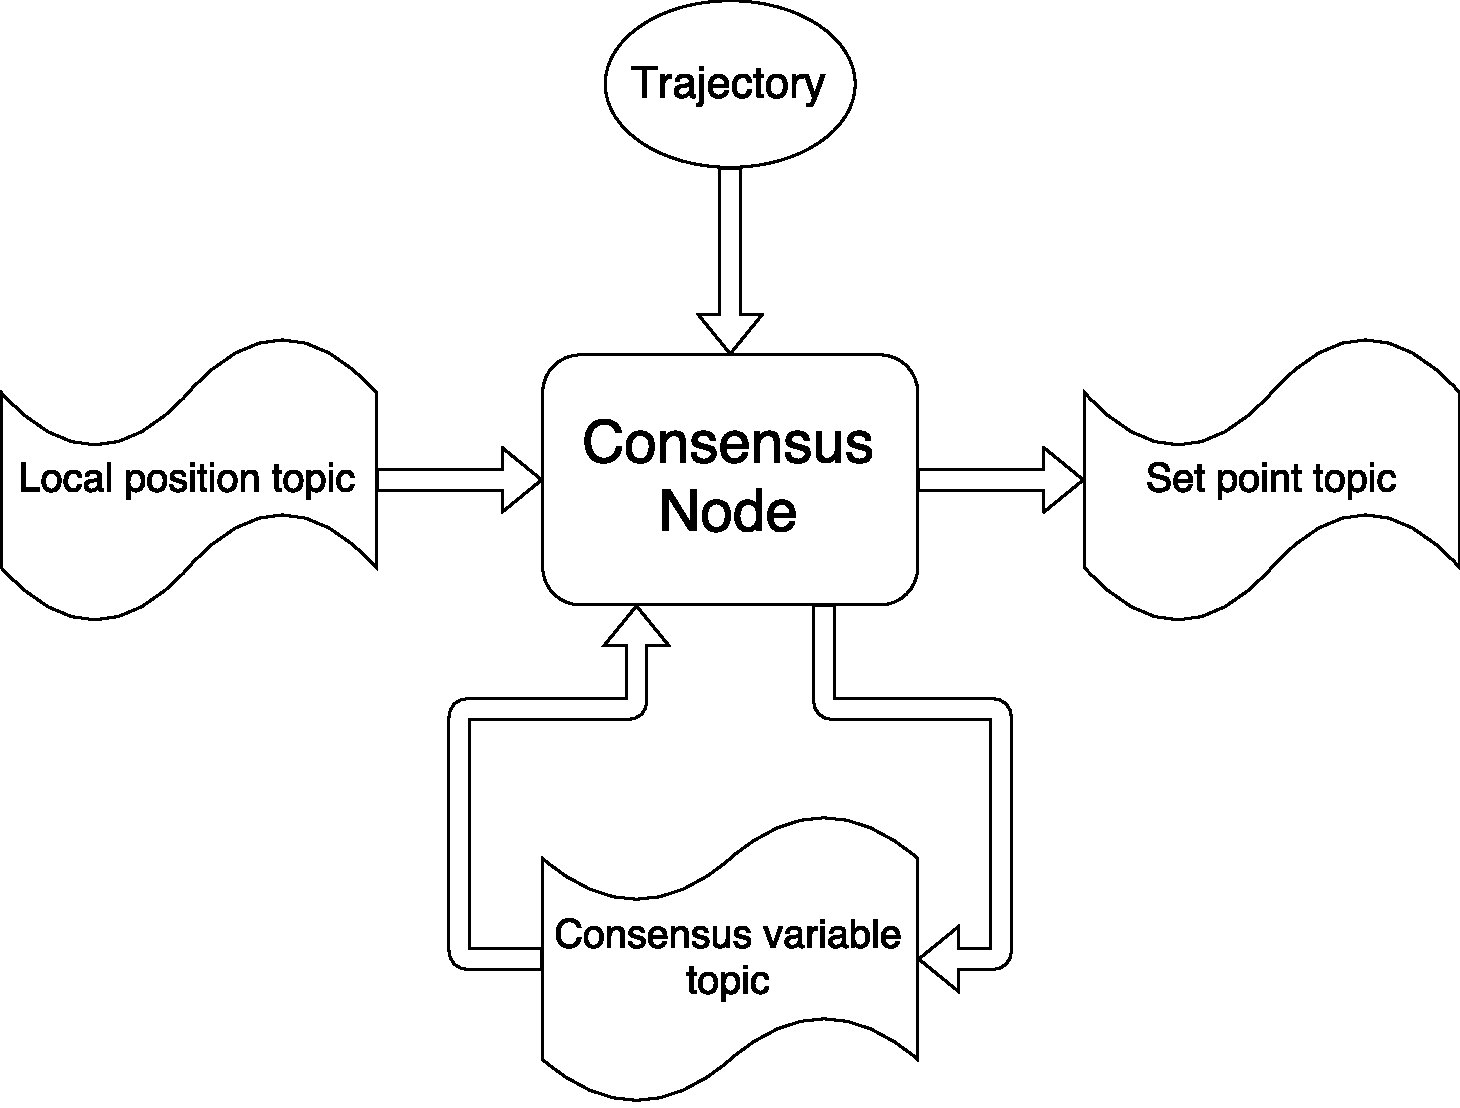
\includegraphics[width=0.9\textwidth]{chapters/chapter-03/figures/consensus_node_structure.pdf}
\caption{Input and output of the node}
\label{fig:node_in_out}
\end{figure}

The subscription of a ROS topic works through a callback function, which accepts as
parameter the pointer to the new message. Since in our case we have multiple subscriptions
and we must advertise the start and stop services, we need to implement a multithreading
architecture which takes care of the concurrent accesses to the state of our object.
The number of threads used is three and these are their functions:
\begin{itemize}
  \item Start and stop services
  \item Consensus variable callback
  \item Local position callback
\end{itemize}

%% Sections of the chapter
\section{Start and stop services\label{sec:start_stop_services}}

First of all, the node can work in two different modes:
\begin{itemize}
  \item trajectory-only
  \item consensus
\end{itemize}

In the trajectory-only mode, the node computes the next set point and sends it to
the UAV, without taking care if there are others UAVs in the mission. Its only objective
is to follow the trajectory and reach its final position trying to respect the time
constraints imposed by the trajectory.
Instead, in the consensus mode, the node does the same computation as before, but
it also publishes its consensus variable and reads all the other ones.
It then considers this information and adjusts its variable.
The consensus mode includes the trajectory-only, and can be started even if the
trajectory-only is already started, while the opposite is not true. When you stop
the consensus mode, also the trajectory-only is stopped.
When the mission is accomplished, the current active mode is stopped automatically,
so that you can freely restart one of the two modes without the need of stopping
the previous one.

The services are implemented using the ROS Service class which manages the whole
infrastructure needed for calling the service. The call to the service is
synchronous and the caller is blocked until the service function is terminated.
In this case, we offer two services: one for starting and stoping the trajectory-only
mode and the other for the consensus mode.
It is possible to customize the service call in order to pass different number
and types of arguments to the service function and the response can also be
defined.
For the two services we have defined the same parameters that are shown in the figure
\ref{fig:custom_service}.

\begin{figure}[h]
\centering
  \lstinputlisting{chapters/chapter-04/code/FlyartCommandBool.srv}
\caption{Custom service structure}
\label{fig:custom_service}
\end{figure}

The message is composed by two parts: the request and the response.
In the request we need a boolean field in order to know if
we want to start or stop the algorithm. The response consists in a boolean variable
which represents the success of the operation and an exit code which identifies
the eventual problems occurred. The constants for the exit codes are directly specified
in the definition of the service.

The trajectory-only service starts or stops the thread which, taken a local position,
computes the next set point; while the consensus one starts or stops the same
thread as before and the one which retrieves the consensus variables from the other
quadrotors.


\section{Consensus variable callback\label{sec:consensus_variable_callback}}

The thread responsible for collecting the consensus variables of all the other UAVs,
is managed by ROS and it executes a callback function when a new message is published
on a specific topic.
This topic is used by all the drones to publish their consensus variable, $\gamma_i$,
and it accepts a custom message which contains only a string with the name of the
owner of the variable and the value itself. The message has also a header, which contains
general information such as timestamp or message id.
The structure of the message can be seen in the figure \ref{fig:custom_message}.

\begin{figure}[h]
\centering
  \lstinputlisting{chapters/chapter-03/code/GammaMsg.msg}
\caption{Custom message structure}
\label{fig:custom_message}
\end{figure}

The callback function receives the information from the topic and updates a local
view of the variables of the neighbors. This information has a timeout validity,
because we do not want to consider too old values. Indeed, if we consider too old
values and a problem in the network causes a loss of packets, our drone might
think which the other drones have a significantly different values of the consensus variables
and so, wait for them. On the contrary, it is better to discard the values and
remove the neighbors after a timeout.

In order to store the information, we use a support class, thread safe, which
provides a procedure to check if the variable is expired or not.
The signatures of the methods of the class are presented in the figure
\ref{fig:consensuss_variable_class}.
We use a container to store the values of the neighbors and we always check if the
value is expired or not before using it.

\begin{figure}[ht]
\centering
  \lstinputlisting[language=C++]{chapters/chapter-03/code/GammaParameter.cpp}
\caption{Consensus variable class}
\label{fig:consensuss_variable_class}
\end{figure}

These variables are used in the consensus law %%TODO reference
as $\gamma_j$ of the neighbors and are used to compute the proportional error.
We can see that the the expiration interval of the values can model the
fact that the network topology can change.
Indeed, if a link between two drones vanished because, for instance, they are
too far from each other, after a timeout (which it is equal to the expiration time),
the neighbor will be removed from the container and the drone will not take into
account the old neighbor.
Even a failure of a drone is ignored using the timeout: if a machine has a critical
problem and does not send its consensus variable, the other drones remove it from
their neighbors and, therefore, they can continue their mission without problems.


\section{Local position callback\label{sec:local_position_callback}}

In the position callback function we apply the consensus law. First of all, we
store the actual position of the drone in an object of a custom class,
which signature is presented in figure \ref{fig:drone_pose}.
\begin{figure}[ht]
\centering
  \lstinputlisting[language=C++]{chapters/chapter-03/code/drone_pose.hpp}
\caption{Class used to manage the position and velocity of the drones}
\label{fig:drone_pose}
\end{figure}
In this class, we also include, besides x, y and z, the yaw of our vehicle. Indeed,
all the operations defined over the class consider also the orientation.

Now, we compute the synchronization term which corresponds to the sum of the
difference between the current $\gamma_i$ and all the $\gamma_j$ of the neighbors.
In order to do this, we iterate over a container, which stores the values, and
we incrementally form the synchronization term.

The next step is to form the $\overline{\alpha}_i$ term.
First of all, we need the next set point, which must be obtained evaluating
the trajectory with the actual value of $\gamma_i$.
Our trajectory is represented by a class, and its signature is shown in the figure
\ref{fig:trajectory}.
\begin{figure}[ht]
\centering
  \lstinputlisting[language=C++]{chapters/chapter-03/code/trajectory.hpp}
\caption{Class used to manage a generic trajectory}
\label{fig:trajectory}
\end{figure}
Now, we simply compute the $position\_error$ as $set\_point - position$.
We also need the desired velocity, which can be obtained using the suitable function
of the trajectory class.
At this point, we have all the terms needed to compute $\overline{\alpha}_i$
as defined in \ref{eq:error_term}.

Since we have all the elements, it is time to apply the consensus law and find
$\ddot{\gamma}_i$. We simply need to have the coefficients $a$ and $b$
and the references $\ddot{\gamma}_d$ and $\dot{\gamma}_d$.

One of the last step needed is the update of $\dot{\gamma}_i$ using $\ddot{\gamma}_i$
and $\gamma_i$ using $\dot{\gamma}_i$. We compute the interval of time, $dt$, between the
last update and the current update and we do the math as:
\begin{lstlisting}
    dgamma += ddgamma * dt;
    gamma += dgamma * dt;
\end{lstlisting}

At the end, we need to publish the value of $\gamma_i$ to the right topic only
if we are operating in consensus mode, otherwise we ignore it. An operation which is
always needed is the publication of the setpoint message to the autopilot of
the UAV, in order to allow it to follow the trajectory and reach its final destination.

